% !TeX root = ./main.tex
\documentclass[main]{subfiles}
\begin{document}
\chapter{Плоскость в пространстве}
$\dim V = 3$
\begin{definition}[Плоскость по 3 точкам]
    Пусть $e_1, e_2, e_3 \in E$, $\vv_1 = \overrightarrow{e_1 e_2}; \vv_2 = \overrightarrow{e_1 e_3}$

    Плоскость -- множество точек $\{e_1 + \alpha\vv_1 + \beta \vv_2: \alpha, \beta \in \R\}$
\end{definition}
\begin{definition}
    Плоскость -- множество решений линейного уравнения:
    \[Ax + By +Cz + D = 0\]
\end{definition}
\begin{theorem}
    Определение 1 равносильно определению 2.
\end{theorem}
\begin{theorem}
    $(A,B,C) = \vn \perp \text{ плоскости}$
\end{theorem}
\begin{proof}
    \begin{gather*}
        e_1 = (x_0, y_0, z_0)\\
        \vn \perp \vv_1 \qquad \vn \perp \vv_2 \qquad \vn = \vv_1 \times \vv_2 \qquad \vn = (A,B,C)\\
        \intertext{$D$ такое число, что}
        Ax_0 + By_0 + Cz_0 + D = 0 \qquad (D = -Ax_0 - By_0 - Cz_0)\\
        - \begin{array}{l}
            Ax + By + Cz + D = 0       \\
            Ax_0 + By_0 + Cz_0 + D = 0 \\
        \end{array}\\
        \begin{array}{l}
            \hline
            A(x - x_0) + B(y - y_0) + C(z - z_0) = 0
        \end{array}\\
        (A;B;C) \cdot (x-x_0, y-y_0, z-z_0) = 0\\
        (x-x_0, y-y_0, z-z_0) = \alpha \vv_1 + \beta \vv_2\\
        (x,y,z) = e_1 + \alpha \vv_1 + \beta \vv_2 \qedhere
    \end{gather*}
\end{proof}

\begin{definition}[Угол между плоскостями]
    \begin{gather*}
        A_1x + B_1 y + C_1 z + D_1 = 0 = \alpha_1\\
        A_2x + B_2 y + C_2 z + D_2 = 0 = \alpha_2\\
        \cos\angle(\alpha_1, \alpha_2) =
        \frac{A_1 A_2 + B_1 B_2 + C_1 C_2}{\sqrt{A_1^2 + B_1^2 + C_1^2}\sqrt{A_2^2 + B_2^2 + C_2^2}}\\
        \alpha_1 \perp \alpha_2: A_1 A_2 + B_1 B_2 + C_1 C_2 = 0\\
        \alpha_1 \parallel \alpha_2: \frac{A_1}{A_2} = \frac{B_1}{B_2} = \frac{C_1}{C_2}
    \end{gather*}
\end{definition}

\begin{definition}[Уравнение плоскости в отрезках]
    \[\frac{x}{p} + \frac{y}{q} + \frac{z}{r} = 1\]
    $p,q,r$ -- отрезки высекаемые плоскостью на $OX, OY, OZ$
\end{definition}


\begin{definition}[Нормальное уравнение плоскости]
    \begin{gather*}
        Ax + By + Cz + D = 0 \qquad |:\sqrt{A^2 + B^2 +C^2} \neq 0\\
        A'x + B'y + C'z +D' = 0\\
        A'^2 + B'^2 + C'^2 = 1
    \end{gather*}
\end{definition}

\begin{definition}
    $A', B', C'$ -- направляющие косинусы

    \noindent\begin{minipage}{.45\textwidth}
        \begin{center}
            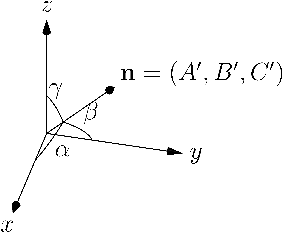
\includegraphics{figures/directional_cosines.pdf}
        \end{center}
    \end{minipage}
    \begin{minipage}{.45\textwidth}
        \begin{gather*}
            A' = \cos \alpha\\
            B' = \cos \beta\\
            C' = \cos \gamma\\
        \end{gather*}
    \end{minipage}
\end{definition}

\begin{theorem}
    \begin{enumerate}
        \item $|D'|$ -- расстояние от $(0,0,0)$ до $\alpha$.
        \item Пусть $Ax + By + Cz + D = 0$ -- плоскость, а $(x_0, y_0, z_0)$ -- точка,
              тогда расстояние от точки до плоскости:
              \[d = \frac{|Ax_0 + By_0 + Cz_0 + D|}{\sqrt{A^2 + B^2 + C^2}}\]
    \end{enumerate}
\end{theorem}
\begin{proof}
    \begin{gather*}
        \intertext{1.} \vn = (A', B', C')\\
        \intertext{$\alpha \vn$ -- конец $\vn$, лежащий в плоскости}
        |\alpha| = d \\
        \alpha \vn = (\alpha A', \alpha B', \alpha C')\\
        A' (\alpha A') + B'(\alpha B') + C'(\alpha C') + D' = 0\\
        \alpha + D' = 0 \qquad |\alpha| = |D'|\\
        \intertext{1.5.}
        (x_0, y_0, z_0) = (0,0,0)\\
        Ax + By + Cz + D = 0\\
        |D'| = \frac{|D|}{\sqrt{A^2+B^2+C^2}} = d\\
        \intertext{2.}
        \tilde{x} = x - x_0 \qquad \tilde{y} = y - y_0 \qquad \tilde{z} = z - z_0\\
        \intertext{Для точки $(x_0, y_0, z_0)$}
        \tilde{x} = x_0 \qquad \tilde{y} = y_0 \qquad \tilde{z} =  z_0\\
        A \tilde{x} + B\tilde{y} + C \tilde{z} + (Ax_0 + By_0 + Cz_0 + D) = 0\\
        d = \frac{|Ax_0 + By_0 + Cz_0 + D|}{\sqrt{A^2+B^2+C^2}}
    \end{gather*}
\end{proof}
\end{document}